\chapter{Manipulating plot rendering with grid}\label{cha:grid}

\section{Introduction}

Sometimes you may need to go beyond the theming system and directly
modify the underlying grid graphics output. To do this, you will need a
good understanding of grid, as described in `R Graphics' (Murrell 2005).
If you can't get the book, at least read Chapter 5, `The grid graphics
model', which is available online for free at
\url{http://www.stat.auckland.ac.nz/~paul/RGraphics/chapter5.pdf}. This
appendix outlines the more important viewports and grobs used by
\texttt{ggplot} and should be helpful if you need to interact with the
grobs produced by \texttt{ggplot}. \index{Grid} \index{Package!grid}

\section{Plot viewports}\label{sec:plot-viewports}

Viewports define the basic regions of the plot. The structure will vary
slightly from plot to plot, depending on the type of faceting used, but
the basics will remain the same. \index{Viewports}
\index{Grid!viewports}

The \texttt{panels} viewport contains the meat of the plot: strip
labels, axes and faceted panels. The viewports are named according to
both their job and their position on the plot. A prefix (listed below)
describes the contents of the viewport, and is followed by integer x and
y position (counting from bottom left) separated by \texttt{\_}. Figure
\ref{fig:panelvp} illustrates this naming scheme for a 2 by 2 plot.

\begin{itemize}
\itemsep1pt\parskip0pt\parsep0pt
\item
  \texttt{strip\_h}: horizontal strip labels
\item
  \texttt{strip\_v}: vertical strip labels
\item
  \texttt{axis\_h}: horizontal axes
\item
  \texttt{axis\_v}: vertical axes
\item
  \texttt{panel}: faceting panels
\end{itemize}

\begin{figure}[htbp]
  \centering
    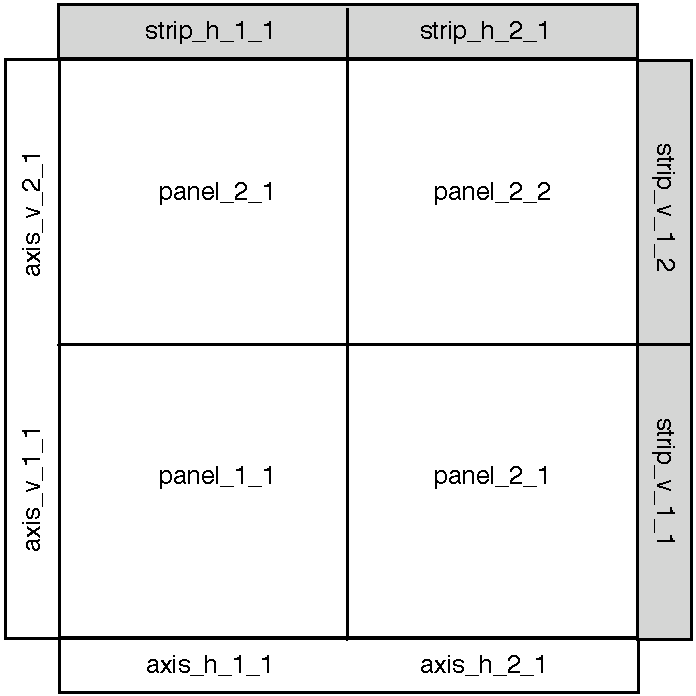
\includegraphics[width=0.5 \linewidth]{diagrams/grid-panelvp}
  \caption{Naming scheming of the panel viewports.}
  \label{fig:panelvp}
\end{figure}

The \texttt{panels} viewport is contained inside the \texttt{background}
viewport which also contains the following viewports:

\begin{itemize}
\itemsep1pt\parskip0pt\parsep0pt
\item
  \texttt{title}, \texttt{xlabel} and \texttt{ylabel}: for the plot
  title, and x and y axis labels
\item
  \texttt{legend\_box}: for all of the legends for the plot
\end{itemize}

Figure \ref{fig:viewports} labels a plot with a representative sample of
these viewports. To get a list of all viewports on the current plot, run
\texttt{current.vpTree(all=TRUE)} or
\texttt{grid.ls(grobs = FALSE, viewports = TRUE)}.

\begin{figure}[htbp]
  \centering
    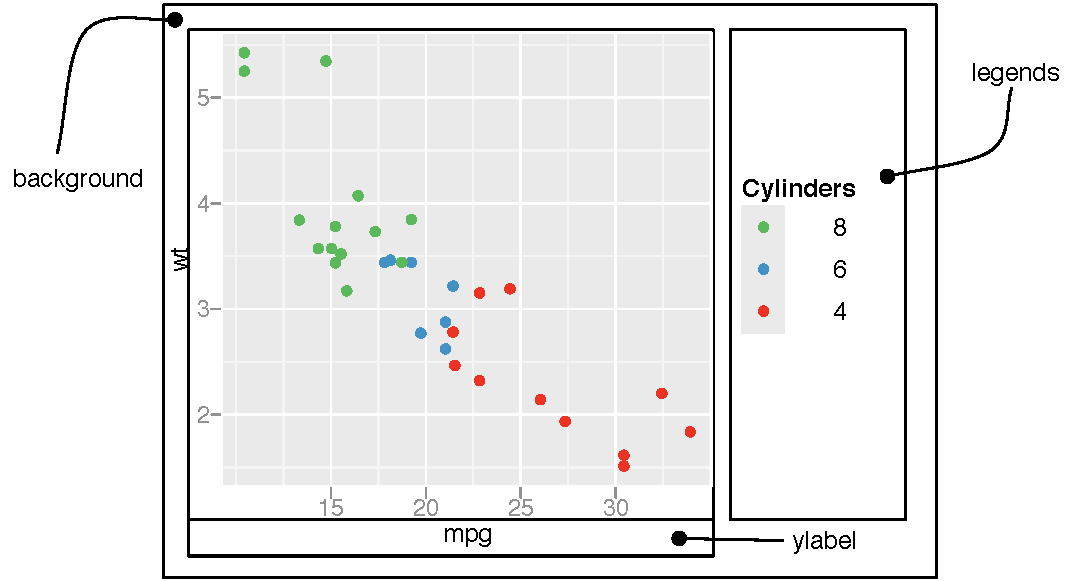
\includegraphics[width=\linewidth]{diagrams/grid-viewports}
  \caption{Diagram showing the structure and names of viewports.}
  \label{fig:viewports}
\end{figure}

\section{Plot grobs}\label{sec:plot-grobs}

Grob names have three components: the name of the grob, the class of the
grob and a unique numeric suffix. The three components are joined
together with \texttt{.} to give a name like \texttt{title.text.435} or
\texttt{ticks.segments.15}. These three components ensure that all grob
names are unique, and allow you to select multiple grobs with the same
name at the same time. Figure \ref{fig:grobs} labels some of these
grobs. The grobs are arranged hierarchically, but it's hard to capture
this in a diagram. You can see a list of all the grobs in the current
plot with \texttt{grid.ls()}. \index{Grid!grobs}

\begin{figure}[htbp]
  \centering
    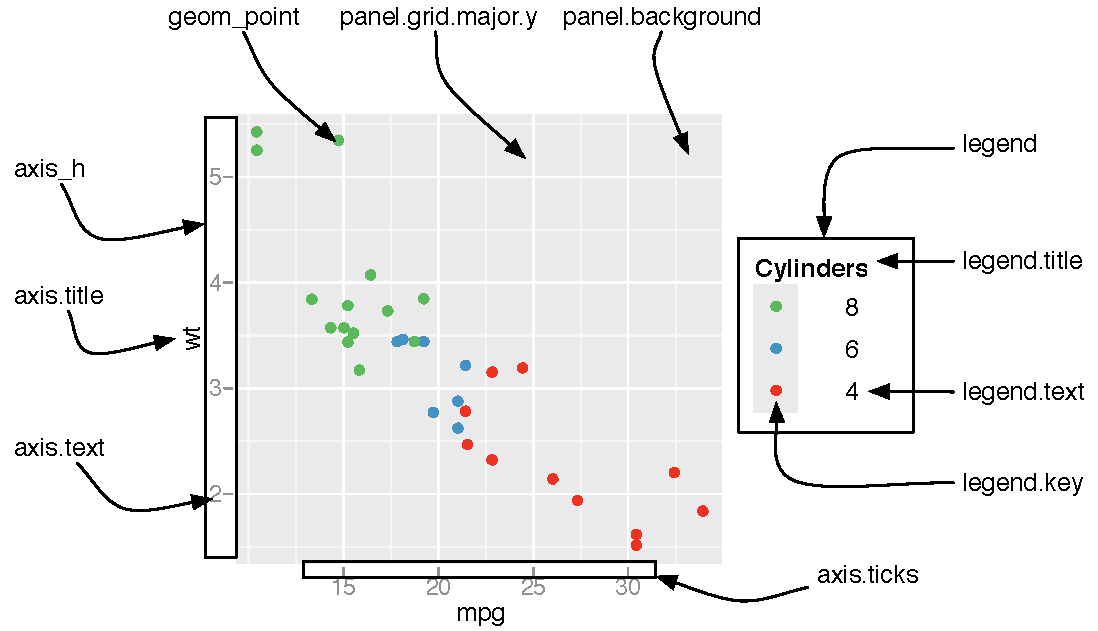
\includegraphics[width=\linewidth]{diagrams/grid-grobs}
  \caption{A selection of the most important grobs.}
  \label{fig:grobs}
\end{figure}

\section{Saving your work}\label{sec:grid-save}

Using \texttt{grid.gedit()}, and similar functions, works fine if you
are editing the plot on screen, but if you want to save it to disk you
need to take some extra steps, or you will end up with multiple pages of
output, each showing one change. The key is not to modify the plot on
screen, but to modify the plot grob, and then draw it once you have made
all the changes. \index{Saving!grid graphics}

\begin{Shaded}
\begin{Highlighting}[]
\NormalTok{p <-}\StringTok{ }\KeywordTok{qplot}\NormalTok{(wt, mpg, }\DataTypeTok{data=}\NormalTok{mtcars, }\DataTypeTok{colour=}\NormalTok{cyl)}
\CommentTok{# Get the plot grob}
\NormalTok{grob <-}\StringTok{ }\KeywordTok{ggplotGrob}\NormalTok{(p)}
\CommentTok{# Modify in place}
\CommentTok{# DEPRECATED!!! seems as though a proper fix hasn't been found}
\CommentTok{# Study this for a solution -- https://groups.google.com/forum/#!topic/ggplot2/iygHrbUNy7w}
\NormalTok{grob <-}\StringTok{ }\KeywordTok{geditGrob}\NormalTok{(grob, }\KeywordTok{gPath}\NormalTok{(}\StringTok{"strip"}\NormalTok{,}\StringTok{"label"}\NormalTok{), }\DataTypeTok{gp=}\KeywordTok{gpar}\NormalTok{(}\DataTypeTok{fontface=}\StringTok{"bold"}\NormalTok{))}

\CommentTok{# Draw it}
\KeywordTok{grid.newpage}\NormalTok{()}
\KeywordTok{grid.draw}\NormalTok{(grob)}
\end{Highlighting}
\end{Shaded}

An alternative is make all of the changes on screen, and then use
\texttt{dev.copy2pdf()} to copy the final version to disk.

Murrell, Paul. 2005. \emph{R Graphics}. Chapman \& Hall/CRC.
